\documentclass{beamer}
\usepackage{t1enc}
\usepackage[utf8]{inputenc}
\usepackage[magyar]{babel}
\usepackage{amsmath}
\usepackage{mathtools}
\usepackage{graphicx}
\usepackage{multirow}
%\usepackage{relsize}
\usetheme{metropolis}

\definecolor{fsfhu}{RGB}{144,1,0}

\usepackage{hyperref}
\hypersetup{colorlinks,linkcolor=fsfhu,urlcolor=fsfhu}

\title{Az OpenScope projekt}
\date{2018. május 12.}
\author{Meskó Balázs \texorpdfstring{\\}{} FSF.hu Alapítvány}
\institute{Szabad Szoftver Konferencia és Kiállítás 2018}
\titlegraphic{
\includegraphics[width=2cm]{images/fsfhu.png}}
\begin{document}

{
  \setbeamercolor{background canvas}{bg=fsfhu}
  \setbeamercolor{normal text}{fg=white}
  \setbeamercolor{title graphic}{fg=white}
  \maketitle
}

  \section{Projektek}
  
  \begin{frame}{GNOME Projekt}
    \begin{center}
    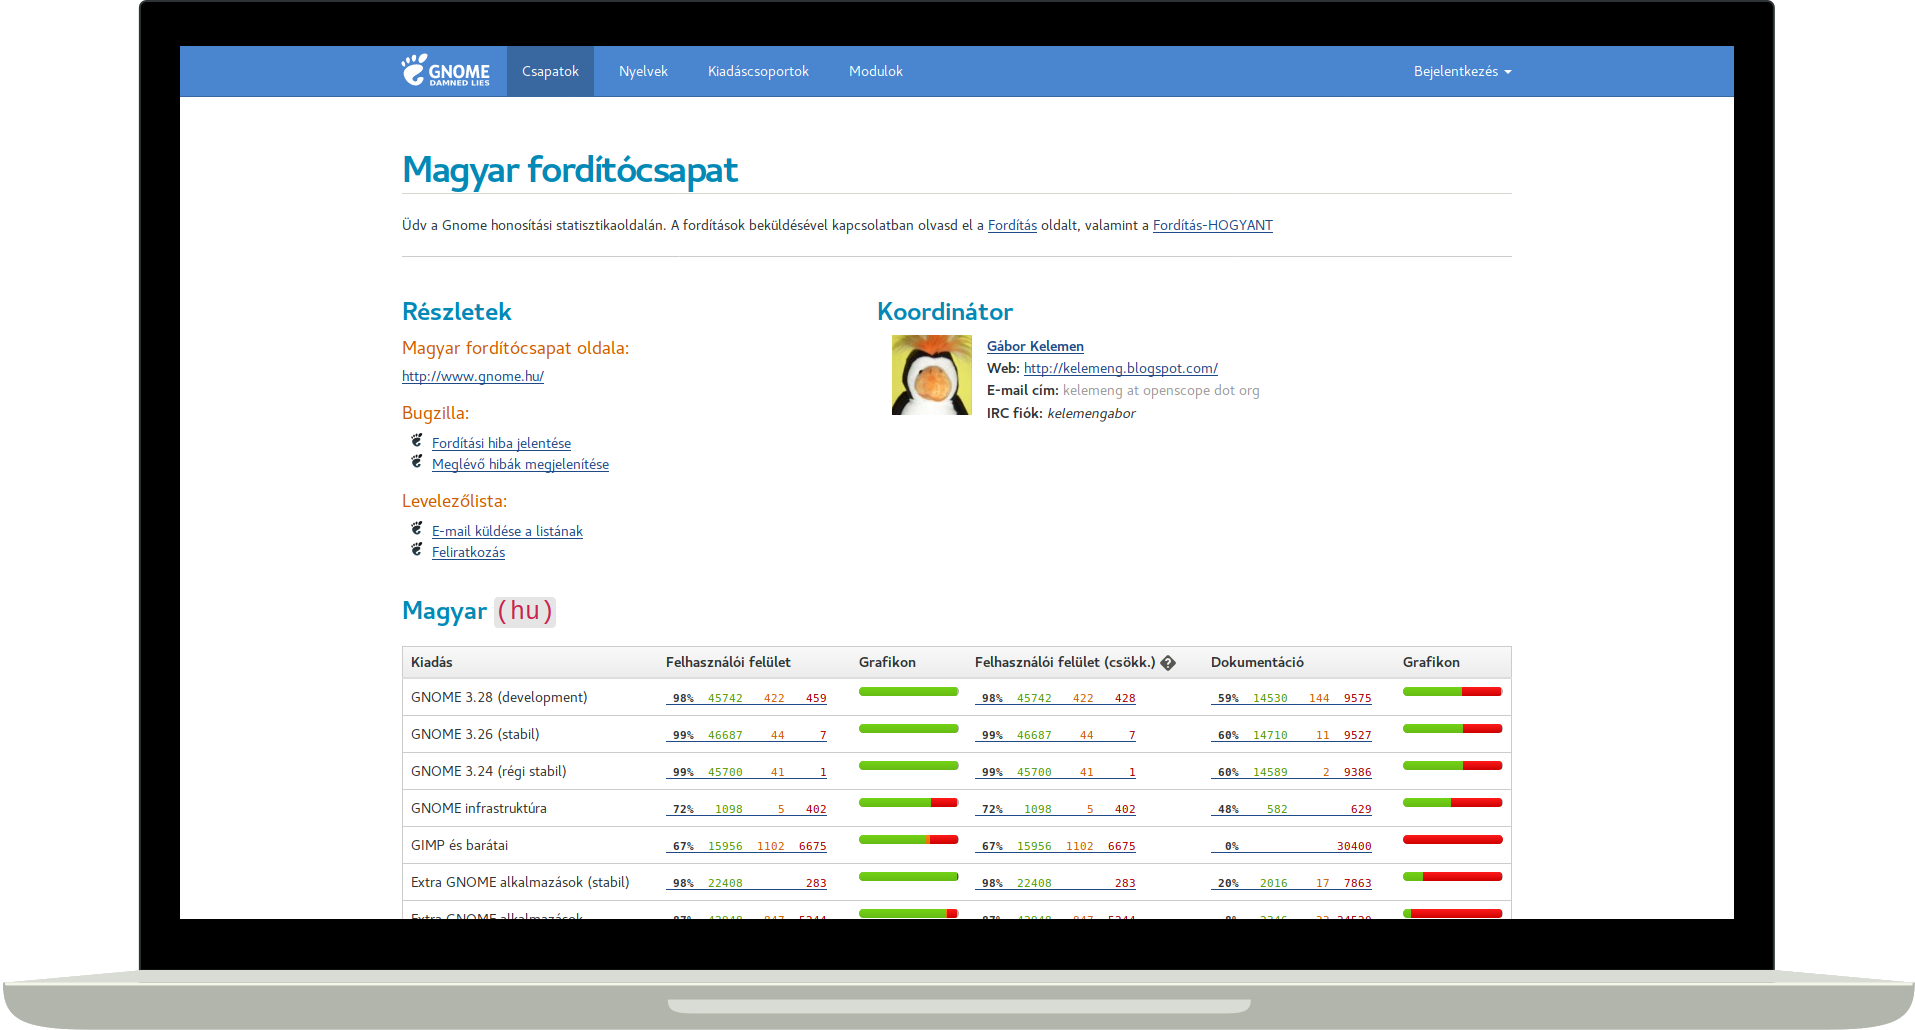
\includegraphics[width=10cm]{images/gnome-laptop.png}
    \end{center}
  \end{frame}

  \begin{frame}{Translation Project}
    \begin{center}
      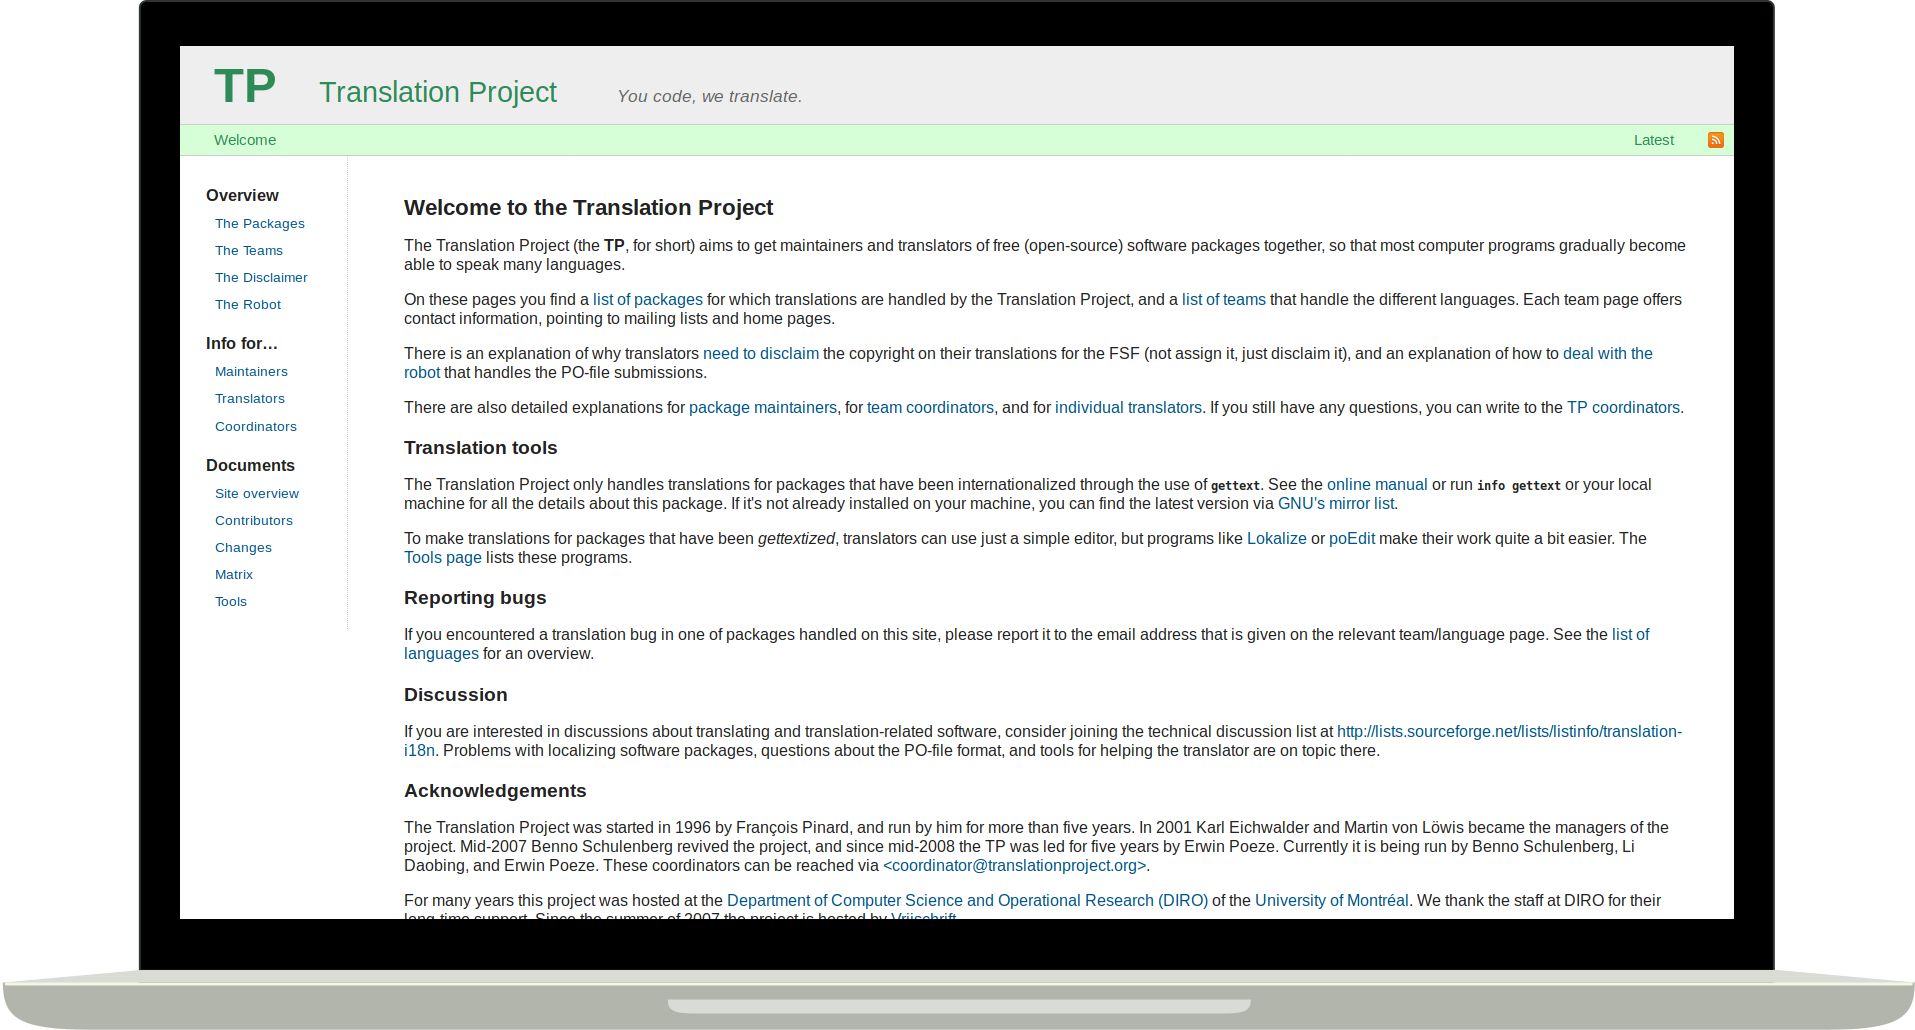
\includegraphics[width=10cm]{images/tp-laptop.png}
    \end{center}
  \end{frame}

  \begin{frame}{Fedora Zanata}
    \begin{center}
      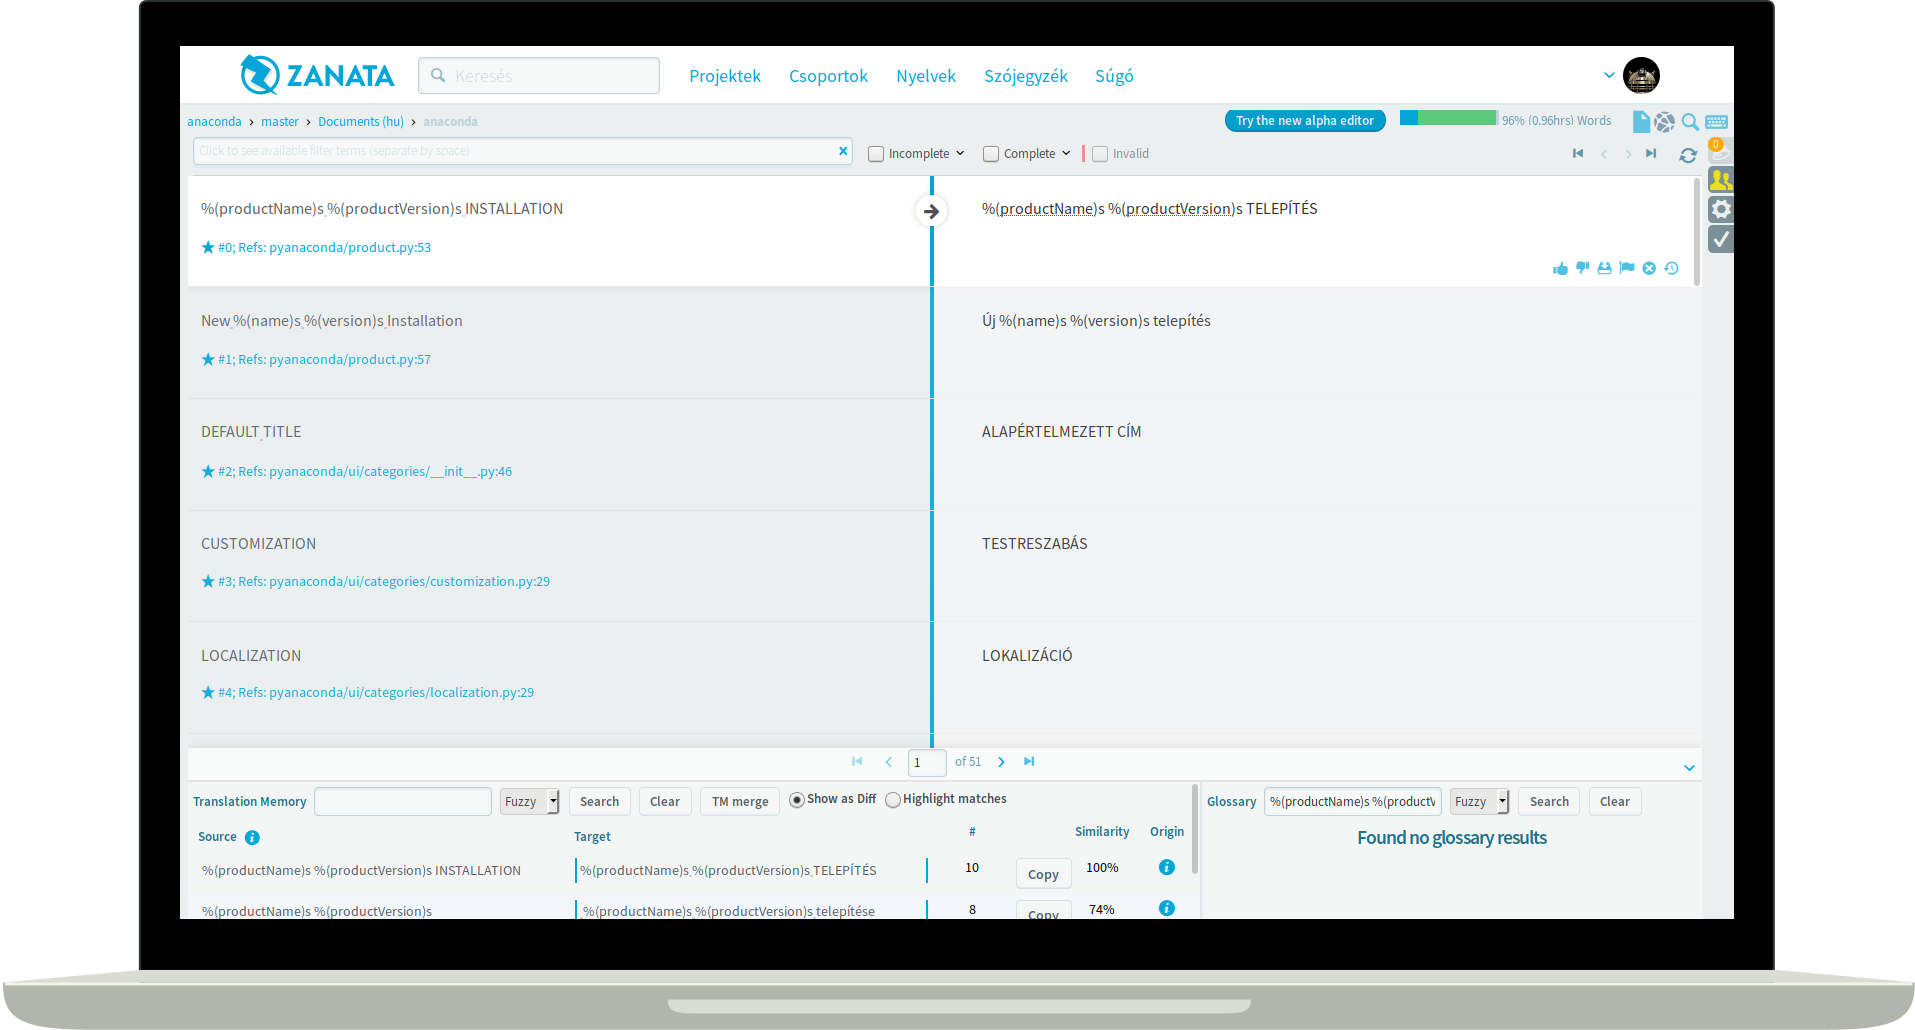
\includegraphics[width=10cm]{images/fedora-zanata-laptop.png}
    \end{center}
  \end{frame}

  \begin{frame}{Továbbiak}
   \begin{itemize}
     \item Transifex
     \item Mozilla Pontoon
     \item Weblate
     \item KDE
     \item …
   \end{itemize}
  \end{frame}

  \begin{frame}[standout]
    
\includegraphics[width=7.5cm]{images/openscope-white.png}
  \end{frame}

  \section{OpenScope.org}

  \begin{frame}{Szolgáltatások}
    \begin{itemize}
      \item OTRS – hibabejelentés, Q\&A
      \item Szójegyzék – OpenScope szótár 2.0 (folyamatban)
      \item Tananyag – Fordítás HOGYAN 2.0 (folyamatban)
      \item Közösség
        \begin{itemize}
          \item Telegram csoport
          \item OpenScope esték \textasciitilde kéthetente
        \end{itemize}
    \end{itemize}
  \end{frame}

  \begin{frame}{Új weboldal}
    \begin{itemize}
      \item Jelenleg fejlesztés alatt
      \item Legfontosabb funkciók:
        \begin{itemize}
          \item OpenScope szótár
          \item Projektfelelősök listája
        \end{itemize}
      \item Nem fórum, sem közösségi oldal(!)
    \end{itemize}
  \end{frame}

  \begin{frame}{Eddigi eredmények}
    \begin{itemize}
      \item Új tagok
      \item Fordítás
        \begin{itemize}
          \item Qt fordítás
          \item Inkscape
        \end{itemize}
    \end{itemize}
  \end{frame}

  \begin{frame}{Közreműködés}
    \begin{itemize}
      \item Fordítás
      \begin{itemize}
        \item Fordítanék, de mit?
        \item Fordítanék, de hogyan?
        \item Fordítanék, de hol?
      \end{itemize}
      \item Tananyagkészítés
      \item Jegykezelés, támogatás
      \item Fejlesztés – főleg PHP
      \begin{itemize}
        \item Szótár: keretprogram, webfelület…\footnote{akár: böngészőbővítmény, asztali integráció}
        \item Statisztika és vizualizáció
      \end{itemize}
      \item{Cikkírás, közösségi média, PR}
    \end{itemize}
  \end{frame}

  \begin{frame}{Hivatkozások}
    \begin{itemize}
      \item \href{http://openscope.org}{openscope.org} avagy \href{http://otrs.fsf.hu}{otrs.fsf.hu}
      \item \href{https://github.com/fsfhu}{github.com/fsfhu}
      \begin{itemize}
        \item Weboldal: \href{https://github.com/fsfhu/openscope-web}{openscope-web}
        \item Szójegyzék: \href{https://github.com/fsfhu/glossary}{glossary}
      \end{itemize}
    \end{itemize}
  \end{frame}

\end{document}